\clearpage
\section{Résultats intermédiaires du 26 septembre 2026 (UTC)}
\subsection{État accepté à 6,2875 secondes}
L'instantané documentaire du 26 septembre à 14 h 46 UTC (10 h 46 EDT)
s'arrête au pas accepté 488; l'horizon prévu reste
\SI{7}{s}. Aucun résultat futur du solveur n'est inclus. Une seule rangée a
été supprimée : \SI{0.01984375}{mm} retirés et \SI{4.74265625}{mm} encore
présents géométriquement. Cette épaisseur restante n'est pas nécessairement
du matériau vierge. La température moyenne de face chaude atteint
\SI{1518.25}{\celsius}. Le maximum nodal exporté vaut aussi
\SI{1518.25}{\celsius} à cette précision; la conversion maximale locale vaut
\(\alpha_{\max}=1\), sans impliquer une conversion totale du liner. Moyenne de face et maximum nodal restent
deux grandeurs distinctes.

\begin{figure}[H]\centering
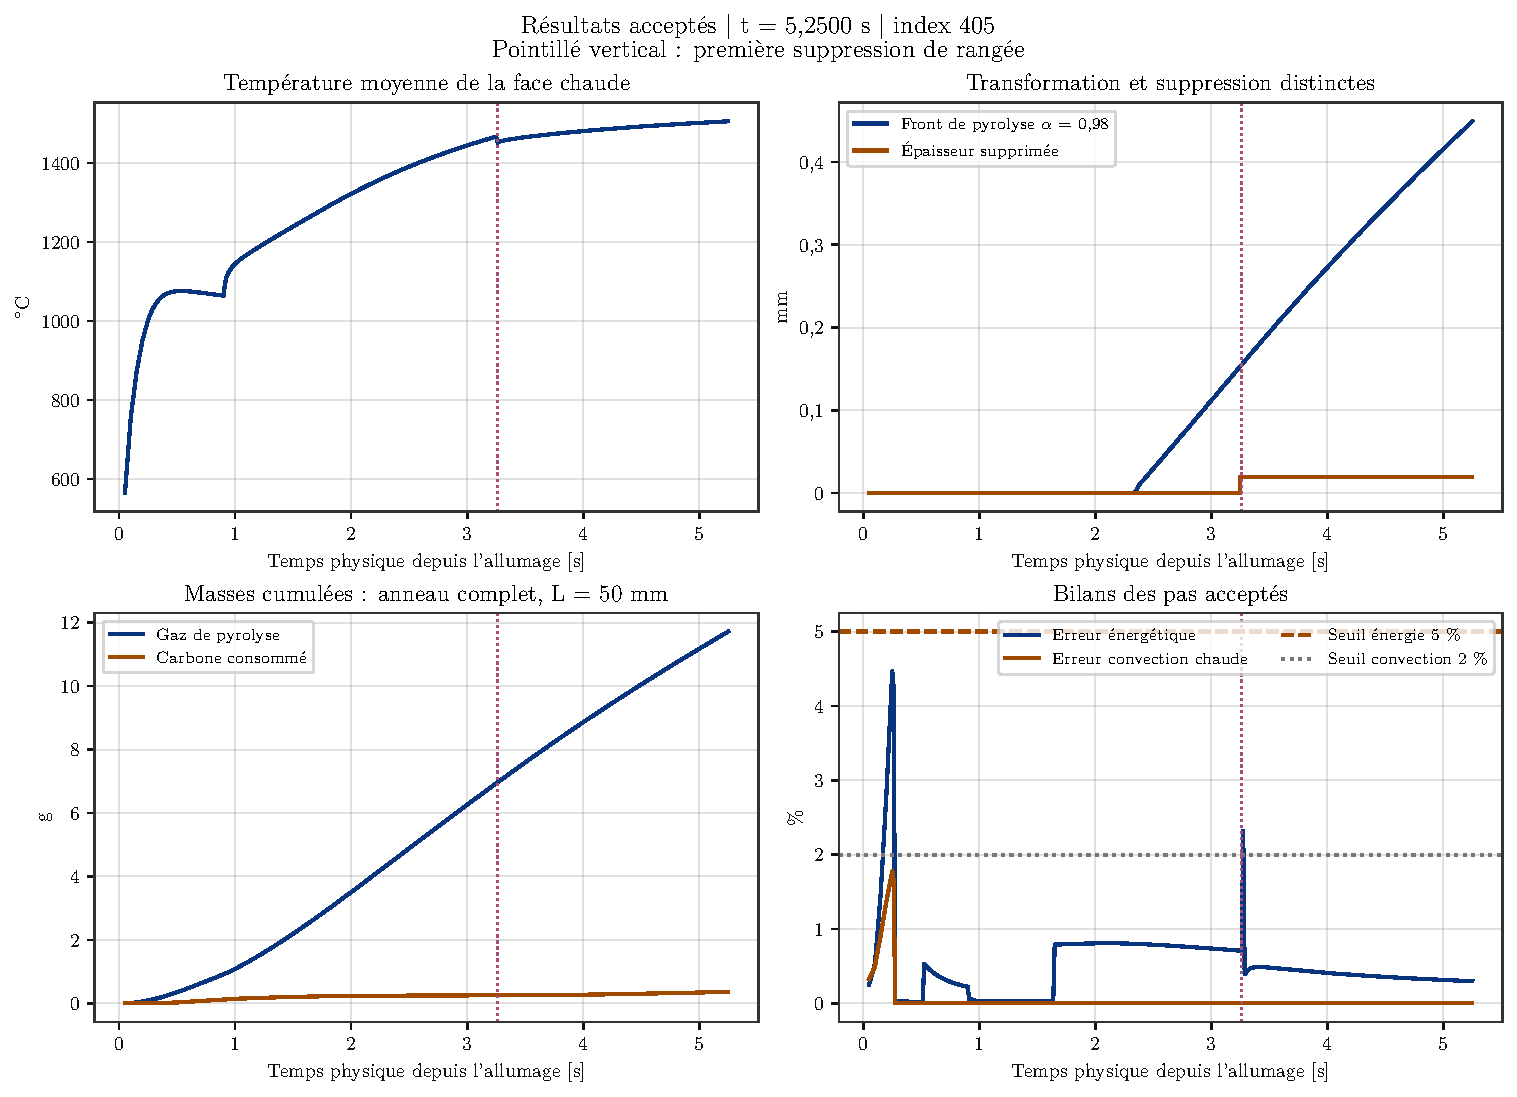
\includegraphics[width=.98\textwidth]{../analysis/newmotor_results_fr.pdf}
\caption{Historique accepté : température moyenne de face chaude, profondeur
pyrolysée et suppression géométrique, masses cumulées et erreurs de bilans.
Les masses sont ramenées à un anneau complet de longueur \SI{50}{mm}.
Le pointillé vertical indique la première suppression de rangée.}
\end{figure}

Au dernier état, l'erreur énergétique relative est de 0,2406\,\% (seuil
5\,\%) et l'erreur relative de convection chaude de \(5.67\times10^{-8}\)
(seuil 0,02). La masse de gaz cumulée vaut \SI{13.8437}{g} et la masse de
carbone consommée \SI{0.47650}{g}, à l'échelle anneau complet. Les audits
acceptés sont tous sous les deux seuils. Cela valide ces contrôles numériques,
pas les lois de matériau exploratoires.

\clearpage
\subsection{Progression du front de pyrolyse}
Pour rester comparable aux estimations précédentes, le front est défini par
\(\bar\alpha\geq0.98\), où \(\bar\alpha\) est la moyenne pondérée par volume
des 500 éléments d'une rangée radiale. On retient la zone continue depuis
l'alésage initial et on interpole linéairement entre centres des rangées qui
encadrent le seuil. Les rangées déjà supprimées gardent leur dernière conversion
acceptée dans cette mesure depuis l'alésage initial.

\begin{figure}[H]\centering
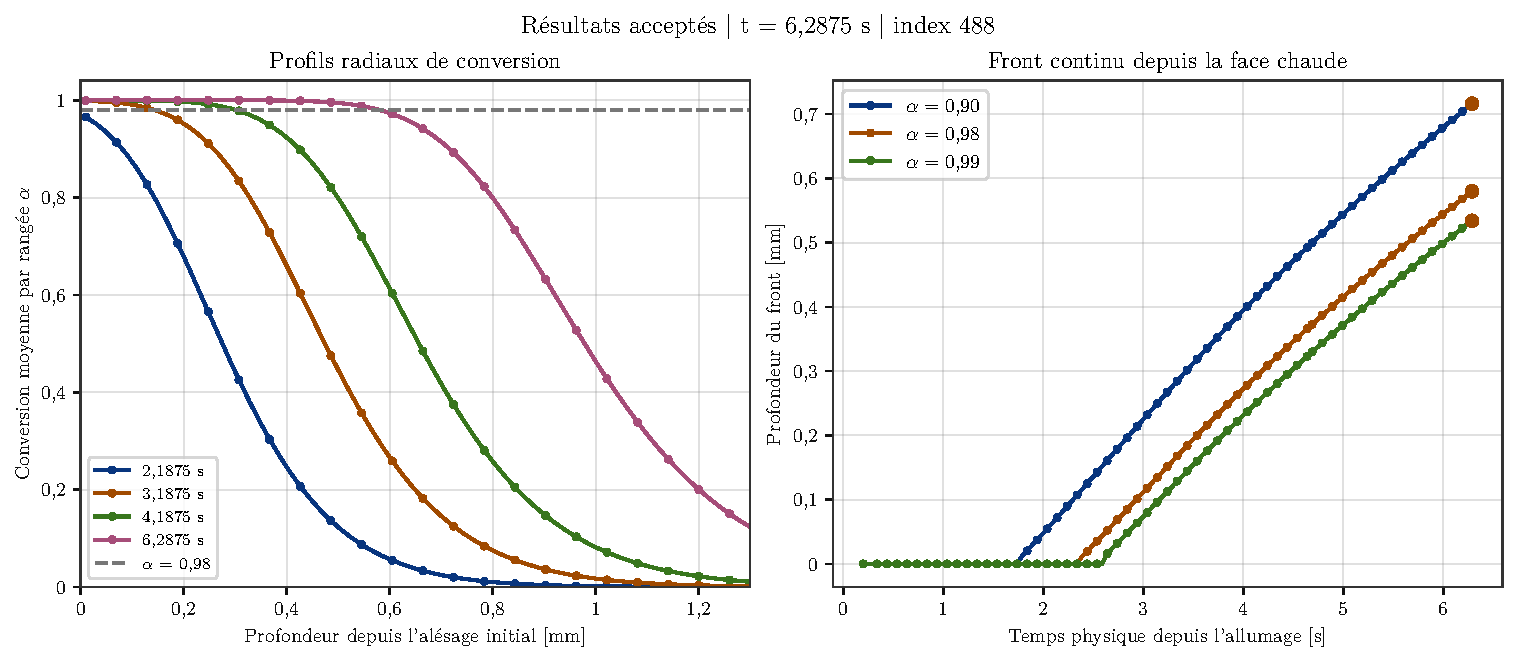
\includegraphics[width=.98\textwidth]{../analysis/newmotor_conversion_fr.pdf}
\caption{Profils de conversion et profondeurs des fronts à 90, 98 et 99\,\%.
Les profils montrent les premiers \SI{1.3}{mm} des \SI{4.7625}{mm} initiaux.
Les historiques des fronts utilisent un checkpoint sur quatre, complété par
le dernier état accepté et le checkpoint de comparaison précédent.}
\end{figure}

À \SI{6.2875}{s}, le front à 98\,\% est à \SI{0.57986}{mm}, soit
12,18\,\% de l'épaisseur initiale. Les fronts à 90 et 99\,\% sont respectivement
à \SI{0.71616}{mm} et \SI{0.53394}{mm}. Le seuil est une définition de
post-traitement : il ne modifie ni la loi de matériau ni la règle de suppression.
\textbf{Pyrolysé ne signifie donc ni brûlé ni géométriquement disparu.}

\clearpage
\subsection{Projections 25, 50 et 75 pour cent}
Une droite est ajustée par moindres carrés à la profondeur du front à 98\,\%
sur les dernières \SI{0.6625}{s} disponibles, avec le même échantillonnage.
L'ajustement actuel utilise 14 points de \SI{5.6375}{s} à \SI{6.2875}{s}.
La vitesse ajustée est \SI{0.12370}{mm.s^{-1}}, contre
\SI{0.12822}{mm.s^{-1}} au précédent rapport à \SI{5.8875}{s} (index 456).

\begin{table}[H]\centering
\caption{Temps physiques depuis l'allumage, et non durées de calcul.}
\begin{tabular}{lrrr}\toprule
Épaisseur initiale pyrolysée & Précédent [s] & Actualisé [s] & Variation\\\midrule
25\,\% & 11,03 & 11,22 & +1,7\,\%\\
50\,\% & 20,32 & 20,85 & +2,6\,\%\\
75\,\% & 29,60 & 30,47 & +2,9\,\%\\\bottomrule
\end{tabular}
\end{table}

\begin{figure}[H]\centering
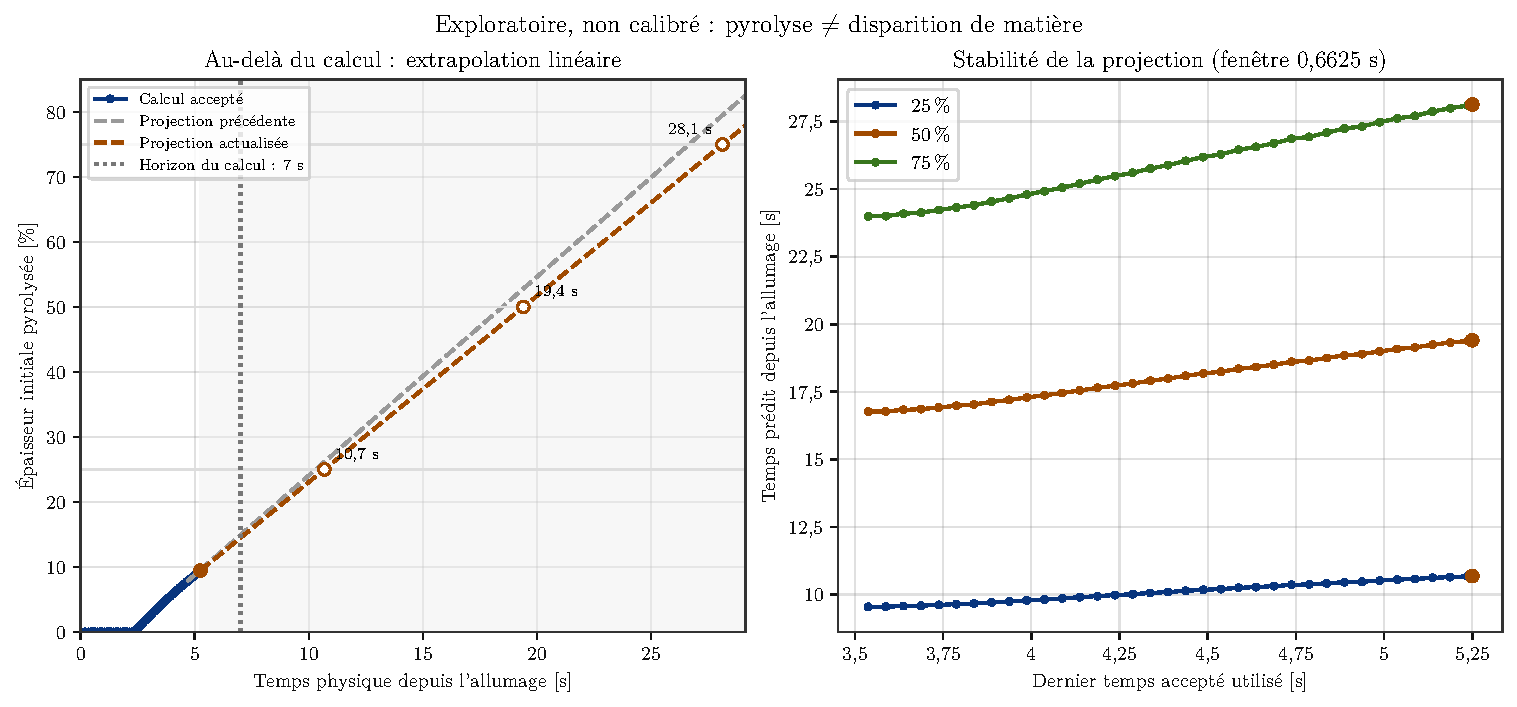
\includegraphics[width=.98\textwidth]{../analysis/newmotor_projections_fr.pdf}
\caption{À gauche, calcul accepté en trait plein et extrapolations en tirets;
la zone grise est au-delà des résultats disponibles. À droite, dérive des temps
prédits lorsque de nouveaux checkpoints entrent dans la fenêtre d'ajustement.}
\end{figure}

La projection à \SI{7}{s} est d'environ 14,03\,\% pyrolysés. Les estimations
25/50/75\,\% augmentent de 1,7 à 2,9\,\% depuis le rapport précédent,
avec le ralentissement du front. Cette dérive ne démontre pas une convergence
prédictive.
Tous ces franchissements sont au-delà de l'horizon actuellement autorisé.
Ce sont des extrapolations linéaires non calibrées, sans intervalle de confiance
physique; elles ne démontrent pas la tenue du moteur. Leur incertitude augmente
fortement à 50 et 75\,\%.

\clearpage
\subsection{Estimation de fin du calcul à 7 secondes}
Au pas accepté 488 à \SI{6.2875}{s}, il reste 57 pas macros de
\SI{0.0125}{s}, soit \SI{0.7125}{s} physiques. Les dix rangs sont actifs;
le pas 489 à \SI{6.3}{s} est convergé mais encore en finalisation.
Son travail n'est pas compté comme accepté. Aucune nouvelle erreur ni
suppression de rangée n'est observée.

La cadence est calculée à partir des dates de modification des audits acceptés,
sur les 10, 20 et 30 derniers intervalles entre pas ordinaires acceptés après
la reprise, terminant au pas 488. La récupération du pas 424 et l'intervalle
de première acceptation du pas 425 sont exclus. Aucune durée d'arrêt, ni l'âge
du pas en cours, n'est déduite du travail restant. Les lenteurs ultérieures
restent incluses. Les dates ci-dessous partent de l'instantané à 10 h 46 EDT
le 26 septembre, à cadence constante.
\begin{table}[H]\centering
\caption{Scénarios à cadence constante au moment de l'instantané.}
\begin{tabular}{lrrl}\toprule
Fenêtre & Minutes/pas & Reste [h] & Fin estimée (EDT)\\\midrule
10 pas & 35,86 & 34,1 & 27 septembre, vers 20 h 50\\
20 pas & 34,14 & 32,4 & 27 septembre, vers 19 h 12\\
30 pas & 40,35 & 38,3 & 28 septembre, vers 01 h 06\\\bottomrule
\end{tabular}
\end{table}
Les six derniers intervalles seuls donnent \SI{36.19}{min} par pas et
environ \SI{34.4}{h} restantes. La fenêtre de 30 pas inclut notamment le long
intervalle de finalisation du pas 467; il n'est pas assimilé ici à du temps CPU.
\textbf{Planification prudente : environ 35 à 50 heures à partir de cet
instantané}, soit du 27 septembre vers 22 h au 28 septembre vers 13 h EDT
(le 28 septembre vers 02 h à 17 h UTC).
Cette enveloppe actualise celle de 65 à 95 heures du rapport au pas 456;
elle repose sur le travail restant et les cadences observées, pas sur une
soustraction du temps écoulé. Ce n'est ni un intervalle de confiance ni une
borne garantie. La cause des variations de cadence n'est pas établie ici;
écritures, exports et suppressions de rangées peuvent encore retarder la fin.
L'estimation concerne uniquement la fin du calcul à \SI{7}{s}, pas la
disparition du liner ni les franchissements extrapolés de 25/50/75\,\%.

\subsection{Sources et reproductibilité}
Le journal \code{newmotor_v0_history.csv} est une vue des audits JSON immuables
de chaque pas accepté : temps, épaisseurs, masses, température de surface,
conversion, charges et bilans. Les figures utilisent directement les audits
acceptés et les checkpoints de conversion, jamais un pas encore en cours
d'export. L'instantané réduit et les empreintes SHA-256 des sources sont dans
\path{docs/analysis/accepted_results_snapshot.json}. Le script
\code{make_results_figures.py} régénère les figures hors ligne; son option
\code{--capture} lit le runtime sans modifier le calcul. Les textes et tableaux
de cette édition sont figés au même index 488. Les horodatages et les trois
scénarios de durée sont également conservés dans cet instantané.
\clearpage
